%%%%%%%%%%%%%%%%%%%%%%%%%%%%%%%%%%%%%%%%%%%%%%%%%%
%% ICN2 pocketbook environments
%%%%%%%%%%%%%%%%%%%%%%%%%%%%%%%%%%%%%%%%%%%%%%%%%%




%%%%%%%%%%%%%%%%%%%%%%%%%%%%%%%%%%%%%%%%%%%%%%%%%%
%% PART1 - The Setting
%%%%%%%%%%%%%%%%%%%%%%%%%%%%%%%%%%%%%%%%%%%%%%%%%%

\newpart{part1}
\rowcolors{1}{part1!10}{white}
\clearpage

%% Economy %%%%%%%%%%%%%%%%%%%%%%%%%%%%%%%%%%%%%%%%%%%

\begin{knitrout}
\definecolor{shadecolor}{rgb}{0.969, 0.969, 0.969}\color{fgcolor}\begin{kframe}
\begin{alltt}
\hlkwd{chart_spread}\hlstd{(}\hlkwc{title}\hlstd{=}\hlstr{"Economy"}\hlstd{,}                \hlcom{# Amy you could specify here}
            \hlkwc{LeftTextCode}\hlstd{=}\hlstr{"TXT.P1.ECON.1.1"}\hlstd{,}  \hlcom{# Amy you could specify here}
            \hlkwc{RightTextCode}\hlstd{=}\hlstr{"C.P1.ECON.1.2"}\hlstd{,}   \hlcom{# Amy you could specify here}
            \hlkwc{LeftChartCode}\hlstd{=}\hlstr{"C.P1.ECON.1.3"}\hlstd{,}   \hlcom{# Amy you could specify here}
            \hlkwc{RightChartCode}\hlstd{=}\hlstr{"C.P1.ECON.1.4"}\hlstd{,}  \hlcom{# Amy you could specify here}
            \hlkwc{BottomChartCode}\hlstd{=}\hlstr{"C.P1.ECON.1.5"}\hlstd{,} \hlcom{# Amy you could specify here}
            \hlkwc{MapCode}\hlstd{=}\hlstr{"M.P1.ECON.1.6"}\hlstd{)}         \hlcom{# Amy you could specify here}
\end{alltt}
\end{kframe}
\end{knitrout}

%% Population %%%%%%%%%%%%%%%%%%%%%%%%%%%%%%%%%%%%%%%%%%%

\begin{knitrout}
\definecolor{shadecolor}{rgb}{0.969, 0.969, 0.969}\color{fgcolor}\begin{kframe}
\begin{alltt}
\hlkwd{chart_spread}\hlstd{(}\hlkwc{title}\hlstd{=}\hlstr{"Population"}\hlstd{,}                               \hlcom{# Amy you could specify here}
            \hlkwc{LeftTextCode}\hlstd{=}\hlstr{"P1.OVER.1.1"}\hlstd{,}                        \hlcom{# Amy you could specify here}
            \hlkwc{RightTextCode}\hlstd{=}\hlstr{"MT.P1.OVER.1.2"}\hlstd{,}                    \hlcom{# Amy you could specify here}
            \hlkwc{footnoteRight}\hlstd{=}\hlstr{"Data after 2010 are projections."}\hlstd{,}  \hlcom{# Amy you could specify here}
            \hlkwc{LeftChartCode}\hlstd{=}\hlstr{"C.P1.OVER.1.2"}\hlstd{,}                     \hlcom{# Amy you could specify here}
            \hlkwc{RightChartCode}\hlstd{=}\hlstr{"C.P1.OVER.1.3"}\hlstd{,}                    \hlcom{# Amy you could specify here}
            \hlkwc{BottomChartCode}\hlstd{=}\hlstr{"C.P1.OVER.1.4"}\hlstd{,}                   \hlcom{# Amy you could specify here}
            \hlkwc{MapCode}\hlstd{=}\hlstr{"M.P1.OVER.1.6"}\hlstd{)}                           \hlcom{# Amy you could specify here}
\end{alltt}
\end{kframe}
\end{knitrout}


%%%%%%%%%%%%%%%%%%%%%%%%%%%%%%%%%%%%%%%%%%%%%%%%%%
%% PART2 - Hunger dimensions
%%%%%%%%%%%%%%%%%%%%%%%%%%%%%%%%%%%%%%%%%%%%%%%%%%

\newpart{part2}
\rowcolors{1}{part1!10}{white}
\clearpage


%% Undernourishment  %%%%%%%%%%%%%%%%%%%%%%%%%%%%%%%%%%%%%%%%%%%

\begin{kframe}
\begin{alltt}
\hlkwd{chart_spread}\hlstd{(}\hlkwc{title}\hlstd{=}\hlstr{"Undernourishment"}\hlstd{,}                \hlcom{# Amy you could specify here}
            \hlkwc{LeftTextCode}\hlstd{=}\hlstr{"TXT.P1.IAF.1.1"}\hlstd{,}  \hlcom{# Amy you could specify here}
            \hlkwc{RightTextCode}\hlstd{=}\hlstr{"MT.P1.IAF.1.2"}\hlstd{,}   \hlcom{# Amy you could specify here}
            \hlkwc{LeftChartCode}\hlstd{=}\hlstr{"C.P1.IAF.1.3"}\hlstd{,}   \hlcom{# Amy you could specify here}
            \hlkwc{RightChartCode}\hlstd{=}\hlstr{"C.P1.IAF.1.4"}\hlstd{,}  \hlcom{# Amy you could specify here}
            \hlkwc{BottomChartCode}\hlstd{=}\hlstr{"C.P1.IAF.1.5"}\hlstd{,} \hlcom{# Amy you could specify here}
            \hlkwc{MapCode}\hlstd{=}\hlstr{"M.P1.IAF.1.6"}\hlstd{)}         \hlcom{# Amy you could specify here}
\end{alltt}
\end{kframe}\begin{ChartPage}{ Undernourishment } 
\LeftText{\IfFileExists{./Text/TXT.P1.IAF.1.1.tex}{Undernourishment refers to food intake that is insufficient to meet dietary energy requirements for an active and healthy life. About 805 million people are estimated to be chronically undernourished in 2012–14. This number has fallen by 100 million over the last decade, and by 209 million since 1990-92. Despite progress, the number is still high, and marked differences across regions persist. Latin America and the Caribbean have made the greatest overall progress, with modest progress in sub-Saharan Africa and Western Asia, which have been afflicted by natural disasters and conflict.}{\lipsum[2]}} 
\RightText{\IfFileExists{./Plots/MT.P1.IAF.1.2.tex} 
 
	               {\begin{table} 

	               \caption{Prevalence of undernourishment (percent, 1990-92 and 2012-14)} 

	               \footnotesize
\begin{center}
\begin{tabular}{lrr}
\toprule
  & 1990-92 & 2012-14\\
\midrule
World & 18.7 & 11.3\\
Developing
countries & 23.4 & 13.5\\
Africa & 27.7 & 20.5\\
Asia & 23.7 & 12.7\\
Latin Am. and the Carib. & 15.3 & 6.1\\
Oceania & 15.7 & 14\\
Developed
countries & $<$5.0 & $<$5.0\\
\toprule
\end{tabular}
\end{center}
 
\footnotesize{}  
 

	               \end{table}}} 
 
\LeftChart{\begin{chart} 
 
	               \caption{Asian countries with the highest number of people undernourished in 2012-14 (1990-92 and 2012-14)} 
\IfFileExists{./Plots/C.P1.IAF.1.3.pdf}{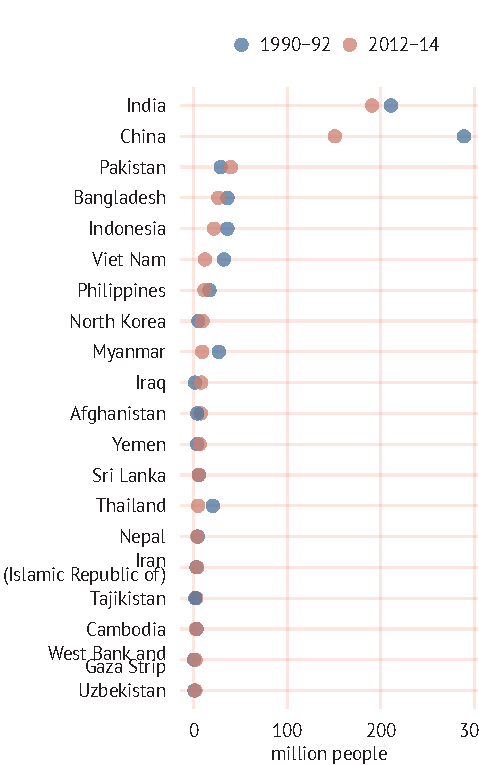
\includegraphics[width = 4cm, height = 8cm]{{./Plots/C.P1.IAF.1.3}.pdf}}{} 
\end{chart}} 
\RightChart{\begin{chart} 
 
	               \caption{African countries with the highest number of people undernourished in 2012-14 (1990-92 and 2012-14)} 
\vspace{-7pt} 
\IfFileExists{./Plots/C.P1.IAF.1.4.pdf}{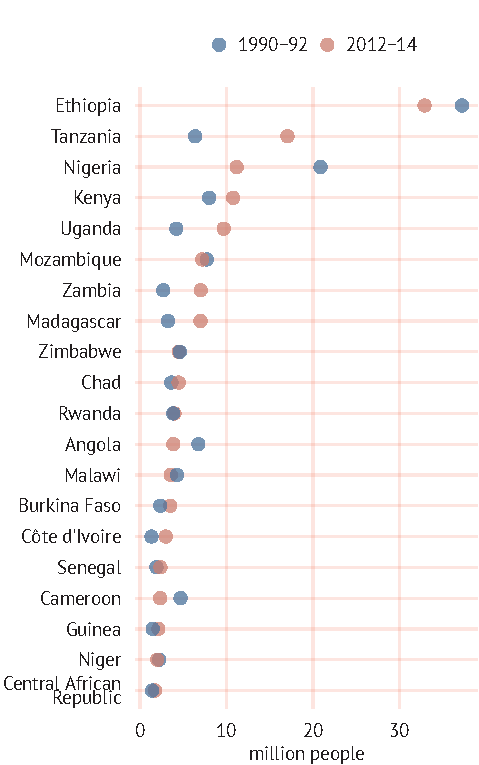
\includegraphics[width = 4cm, height = 8cm]{{./Plots/C.P1.IAF.1.4}.pdf}}{} 
\end{chart}} 
\BottomChart{\begin{chart} 
 
	               \caption{Number of people undernourished (1990-92 to 2012-14)} 
\vspace{-7pt} 
\IfFileExists{./Plots/C.P1.IAF.1.5.pdf}{
\includegraphics[width = 8cm, height = 3cm]{{./Plots/C.P1.IAF.1.5}.pdf}}{} 
\end{chart}} 
\end{ChartPage}\begin{figure} 
\caption{Prevalence of people undernourished (percent, 2014)} 
\IfFileExists{./Maps/M.P1.IAF.1.6.pdf}{\centering
\includegraphics[height = 1\columnwidth, angle=90]{{./Maps/M.P1.IAF.1.6}.pdf}\par}{\newpage\thispagestyle{empty}\mbox{}}{} 
\end{figure}



%%%%%%%%%%%%%%%%%%%%%%%%%%%%%%%%%%%%%%%%%%%%%%%%%%
%% PART3 - Food Supply
%%%%%%%%%%%%%%%%%%%%%%%%%%%%%%%%%%%%%%%%%%%%%%%%%%

\newpart{part3}
\rowcolors{1}{part1!10}{white}
\clearpage


%% Production %%%%%%%%%%%%%%%%%%%%%%%%%%%%%%%%%%%%%%%%%%%

\begin{knitrout}
\definecolor{shadecolor}{rgb}{0.969, 0.969, 0.969}\color{fgcolor}\begin{kframe}
\begin{alltt}
\hlkwd{chart_spread}\hlstd{(}\hlkwc{title}\hlstd{=}\hlstr{"Production"}\hlstd{,}             \hlcom{# Amy you could specify here}
            \hlkwc{LeftTextCode}\hlstd{=}\hlstr{"TXT.P1.ECON.1.1"}\hlstd{,}  \hlcom{# Amy you could specify here}
            \hlkwc{RightTextCode}\hlstd{=}\hlstr{"C.P1.ECON.1.2"}\hlstd{,}   \hlcom{# Amy you could specify here}
            \hlkwc{LeftChartCode}\hlstd{=}\hlstr{"C.P1.ECON.1.3"}\hlstd{,}   \hlcom{# Amy you could specify here}
            \hlkwc{RightChartCode}\hlstd{=}\hlstr{"C.P1.ECON.1.4"}\hlstd{,}  \hlcom{# Amy you could specify here}
            \hlkwc{BottomChartCode}\hlstd{=}\hlstr{"C.P1.ECON.1.5"}\hlstd{,} \hlcom{# Amy you could specify here}
            \hlkwc{MapCode}\hlstd{=}\hlstr{"M.P1.ECON.1.6"}\hlstd{)}         \hlcom{# Amy you could specify here}
\end{alltt}
\end{kframe}
\end{knitrout}


%%%%%%%%%%%%%%%%%%%%%%%%%%%%%%%%%%%%%%%%%%%%%%%%%%
%% PART4 - Sustainability dimensions
%%%%%%%%%%%%%%%%%%%%%%%%%%%%%%%%%%%%%%%%%%%%%%%%%%

\newpart{part2}
\rowcolors{1}{part1!10}{white}
\clearpage

%% Forests %%%%%%%%%%%%%%%%%%%%%%%%%%%%%%%%%%%%%%%%%%%

\begin{knitrout}
\definecolor{shadecolor}{rgb}{0.969, 0.969, 0.969}\color{fgcolor}\begin{kframe}
\begin{alltt}
\hlkwd{chart_spread}\hlstd{(}\hlkwc{title}\hlstd{=}\hlstr{"Forests"}\hlstd{,}                \hlcom{# Amy you could specify here}
            \hlkwc{LeftTextCode}\hlstd{=}\hlstr{"TXT.P1.ECON.1.1"}\hlstd{,}  \hlcom{# Amy you could specify here}
            \hlkwc{RightTextCode}\hlstd{=}\hlstr{"C.P1.ECON.1.2"}\hlstd{,}   \hlcom{# Amy you could specify here}
            \hlkwc{LeftChartCode}\hlstd{=}\hlstr{"C.P1.ECON.1.3"}\hlstd{,}   \hlcom{# Amy you could specify here}
            \hlkwc{RightChartCode}\hlstd{=}\hlstr{"C.P1.ECON.1.4"}\hlstd{,}  \hlcom{# Amy you could specify here}
            \hlkwc{BottomChartCode}\hlstd{=}\hlstr{"C.P1.ECON.1.5"}\hlstd{,} \hlcom{# Amy you could specify here}
            \hlkwc{MapCode}\hlstd{=}\hlstr{"M.P1.ECON.1.6"}\hlstd{)}         \hlcom{# Amy you could specify here}
\end{alltt}
\end{kframe}
\end{knitrout}

